% 线审0910 探针：六片段按 body.tex 同宽置入，一图一页，供矢量属性审计
\documentclass{article}
\pagestyle{empty}
\usepackage{tikz}
\usepackage{graphicx}
\newcommand{\qldrop}{0.649mm}
\newcommand{\qldsub}[1]{\raisebox{-\qldrop}{\fontsize{9.68pt}{9.68pt}\selectfont $#1$}}
\newcommand{\qlabs}[3]{$#1$\kern#3\qldsub{#2}}
\newcommand{\qlab}[1]{$#1$}
\definecolor{cubegray}{gray}{0.25}
\begin{document}
\resizebox{80.8mm}{!}{% g6-triple.tikz —— 片G 0910 集成自 _tmp片G素材/sub3_投影三联.tikz（L37–122 正文，逐字拷入，仅删空行）
% 源图：variantF/media/media/sub3_B_4.png 1408×374px = 源排印宽 86.0mm；画布 86.0000×22.8440mm
% 集成口径：原 body.tex 置入 60mm（缩至 0.698），本片改按栏宽 \linewidth=84.0mm（缩至 0.9767，同比）
% 改名（集成必需）：素材宏 \head → \qlhead（定义 1 处 + 调用 10 处）——\head 与宿主既有同名控制序列冲突
% 依赖：宿主导言 \usepackage{tikz}；\symbfit 由 unicode-math 提供，片段首行 \providecommand 兜底
\providecommand{\symbfit}[1]{\mathbf{#1}}% 纯 tikz 体检回落（unicode-math 在位时本行不生效）
\def\qlhead#1#2{% #1=尖端坐标  #2=指向角（度，TikZ y 向上）
  \begin{scope}[shift={#1},rotate={#2}]%
    \fill (0,0)--(-2.382,0.580)--(-1.924,0)--(-2.382,-0.580)--cycle;%
  \end{scope}}%
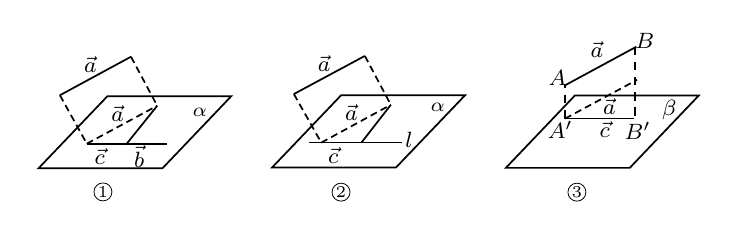
\begin{tikzpicture}[x=1mm,y=1mm,line width=0.22mm,line cap=butt,line join=miter,
                    font=\fontsize{7.86pt}{9.4pt}\selectfont]
  \path[use as bounding box] (0,0) rectangle (86.0000,22.8440);   % bbox＝源画布 1408×374 px
  % ======================= ① 左联 =======================
  % 平面 α：源 px BL(22.44,292.50) BR(280.15,292.50) TR(423.29,142.51) TL(165.76,142.53)
  \draw ( 1.3706, 4.9780) -- (17.1114, 4.9780) -- (25.8544,14.1393) -- (10.1245,14.1381) -- cycle;
  % 虚线链（先画，压在实线之下）：尾-尾、尖-尖、链C（＝向量 a 平移于平面内的虚线拷贝）
  \draw[dash pattern=on 0.880mm off 0.550mm] ( 4.0923,14.2621) -- ( 7.5128, 8.1114); % 链A px(67,140.5)-(123,241.2)
  \draw[dash pattern=on 0.880mm off 0.550mm] (13.1187,19.1539) -- (16.4548,12.9305); % 链B px(214.78,60.41)-(269.4,162.3)
  \draw[dash pattern=on 0.880mm off 0.550mm] ( 7.5128, 8.1114) -- (16.4548,12.9305); % 链C px(123,241.2)-(269.4,162.3)
  % 基线：c 杆 px(123,241.2)→O(206,241.2)；b 杆 O→px(290.5,241.2)（源为一条实拉通线，两处带头）
  \draw ( 7.5128, 8.1114) -- (12.5824, 8.1114);   % c 杆
  \draw (12.5824, 8.1114) -- (17.7436, 8.1114);   % b 杆
  % 面内向量 a：O→px(269.4,162.3)
  \draw (12.5824, 8.1114) -- (16.4548,12.9305);
  % 自由向量 a：px(67,140.5)→(214.78,60.41)（杆线最小二乘拟合 rms 0.2px）
  \draw ( 4.0923,14.2621) -- (13.1187,19.1539);
  % 箭头头部（源 px 尖端）
  \qlhead{(12.5824, 8.1114)}{0}    % c 头，指向 +x（尖端＝O）
  \qlhead{(17.7436, 8.1114)}{0}    % b 头，指向 +x
  \qlhead{(16.4548,12.9305)}{51.22}% 面内 a 头
  \qlhead{(13.1187,19.1539)}{28.46}% 自由 a 头
  % 标签（锚点＝源墨迹盒中心，mm）
  \node[inner sep=0pt] at ( 7.9709,18.1101) {$\vec{\symbfit{a}}$};  % 源盒 px x[119,142] y[61,94]
  \node[inner sep=0pt] at (11.4219,11.9716) {$\vec{\symbfit{a}}$};  % 源盒 px x[175,199] y[161,195]
  \node[inner sep=0pt] at ( 9.1619, 6.4439) {$\vec{\symbfit{c}}$};  % 源盒 px x[139,161] y[252,285]
  \node[inner sep=0pt] at (14.1705, 6.5050) {$\vec{\symbfit{b}}$};  % 源盒 px x[220,244] y[247,288]
  \node[inner sep=0pt,font=\fontsize{7.11pt}{8.5pt}\selectfont] at (21.8665,12.0632) {$\alpha$}; % 源盒 px x[348,368] y[167,186]
  \draw[line width=0.10mm] ( 9.5589, 1.9851) circle[radius=1.1420]; % 圈号① 源圆心 px(156.5,341.5) 外径39px/环宽1.6px
  \node[inner sep=0pt,font=\fontsize{6.29pt}{7.5pt}\selectfont] at (9.5589,1.9851) {1};
  % ======================= ② 中联 =======================
  % 平面 α：源 px BL(508.46,290.50) BR(766.05,290.50) TR(909.45,140.51) TL(651.67,140.57)
  \draw (31.0565, 5.1001) -- (46.7900, 5.1001) -- (55.5488,14.2615) -- (39.8037,14.2578) -- cycle;
  \draw[dash pattern=on 0.880mm off 0.550mm] (33.8075,14.4148) -- (37.2891, 8.2457); % 链A′ px(553.5,138)-(610.5,239)
  \draw[dash pattern=on 0.880mm off 0.550mm] (42.8192,19.2553) -- (46.1212,13.0527); % 链B′ px(701.04,58.75)-(755.1,160.3)
  \draw[dash pattern=on 0.880mm off 0.550mm] (37.2891, 8.2457) -- (46.1212,13.0527); % 链C′ px(610.5,239)-(755.1,160.3)
  % 直线 l（过 O 的水平线，左端 px584.8、右端 px777.5，无箭头）
  \draw (35.7193, 8.2457) -- (47.4893, 8.2457);
  % c 杆：px(610.5,239)→O(694,239)；面内向量 a：O→px(755.1,160.3)；自由 a：px(553.5,138)→(701.04,58.75)
  \draw (37.2891, 8.2457) -- (42.3892, 8.2457);
  \draw (42.3892, 8.2457) -- (46.1212,13.0527);
  \draw (33.8075,14.4148) -- (42.8192,19.2553);
  \qlhead{(42.3892, 8.2457)}{0}    % c 头（尖端＝O）
  \qlhead{(46.1212,13.0527)}{52.18}% 面内 a 头
  \qlhead{(42.8192,19.2553)}{28.24}% 自由 a 头
  \node[inner sep=0pt] at (37.6555,18.2322) {$\vec{\symbfit{a}}$};  % 源盒 px x[605,628] y[59,92]
  \node[inner sep=0pt] at (41.1065,12.0938) {$\vec{\symbfit{a}}$};  % 源盒 px x[661,685] y[159,193]
  \node[inner sep=0pt] at (38.8161, 6.5661) {$\vec{\symbfit{c}}$};  % 源盒 px x[625,646] y[250,283]
  \node[inner sep=0pt,font=\fontsize{7.11pt}{8.5pt}\selectfont] at (52.1009,12.7351) {$\alpha$}; % 源盒 px x[843,863] y[156,175]
  \node[inner sep=0pt] at (48.4361, 8.6122) {$l$};                  % 源盒 px x[788,798] y[218,248]
  \draw[line width=0.10mm] (39.7933, 1.9545) circle[radius=1.1420]; % 圈号② 源圆心 px(651.5,342) 外径39px/环宽1.6px
  \node[inner sep=0pt,font=\fontsize{6.29pt}{7.5pt}\selectfont] at (39.7933,1.9545) {2};
  % ======================= ③ 右联 =======================
  % 平面 β：源 px BL(994.26,291.50) BR(1251.90,291.50) TR(1395.43,141.03) TL(1137.80,141.02)
  \draw (60.7289, 5.0391) -- (76.4655, 5.0391) -- (85.2322,14.2297) -- (69.4963,14.2303) -- cycle;
  % 竖直虚线 A–A′、B–B′（第二档虚线）
  \draw[dash pattern=on 1.100mm off 0.812mm, dash phase=0.611mm] (68.2747,15.6364) -- (68.2747,11.2692); % A–A′ px(1117.8,118)-(1117.8,189.5)
  \draw[dash pattern=on 1.100mm off 0.812mm] (77.1435,20.4250) -- (77.1435,11.2997); % B–B′ px(1263,39.6)-(1263,189)
  % 中斜虚线向量 a′（自 A′ 起、与 a 同向的虚线拷贝，端头带箭头）
  \draw[dash pattern=on 0.880mm off 0.550mm] (68.2564,11.2997) -- (77.3934,16.2166); % px(1117.5,189)-(1267.1,108.5)
  % A′B′ 水平向量：px(1115.5,188.7)→(1261.2,188.7)
  \draw (68.1342,11.3180) -- (77.0335,11.3180);
  % 自由向量 a：A(1118,119.5) → B(1265.6,39.6)
  \draw (68.2869,15.5447) -- (77.3023,20.4250);
  \qlhead{(77.0335,11.3180)}{0}    % A′B′ 头（尖端＝B′）
  \qlhead{(77.3023,20.4250)}{28.43}% 自由 a 头（尖端＝B）
  \qlhead{(77.3934,16.2166)}{28.28}% 中斜 a′ 头
  \node[inner sep=0pt] at (67.2794,16.4304) {$A$};                  % 源盒 px x[1087,1111] y[90,120]
  \node[inner sep=0pt] at (78.3651,21.1641) {$B$};                  % 源盒 px x[1270,1296] y[13,42]
  \node[inner sep=0pt] at (67.6456, 9.8643) {$A'$};                 % 源盒 px x[1089,1126] y[198,229]
  \node[inner sep=0pt] at (77.4797, 9.7422) {$B'$};                 % 源盒 px x[1248,1284] y[199,230]
  \node[inner sep=0pt] at (72.2876,20.0036) {$\vec{\symbfit{a}}$};  % 源盒 px x[1172,1195] y[30,63]
  \node[inner sep=0pt] at (73.8757,12.7656) {$\vec{\symbfit{a}}$};  % 源盒 px x[1198,1221] y[148,182]
  \node[inner sep=0pt] at (73.2955, 9.8949) {$\vec{\symbfit{c}}$};  % 源盒 px x[1189,1211] y[195,229]
  \node[inner sep=0pt] at (81.4801,12.3686) {$\beta$};              % 源盒 px x[1322,1346] y[152,191]
  \draw[line width=0.10mm] (69.7528, 1.9545) circle[radius=1.1420]; % 圈号③ 源圆心 px(1142,342) 外径39px/环宽1.6px
  \node[inner sep=0pt,font=\fontsize{6.29pt}{7.5pt}\selectfont] at (69.7528,1.9545) {3};
\end{tikzpicture}%
% 注：末行 % 必需——\input 时尾随换行会成空格 token，被计入裁切框。
}\newpage
\resizebox{41.1mm}{!}{% g1-prism.tikz —— 片G 0910 集成自 _tmp片G素材/img1_tikz.tex（L42–71 片段正文，逐字拷入，仅删空行、末行加 %）
% 源图：variantF/media/media/image1.png 691×1159px = 41.100×68.936mm（源排印宽 41.1mm）
% 依赖：宿主导言 \usepackage{tikz} + 宏 \qldrop/\qldsub/\qlabs/\qlab（见 qp-blocks.tex）
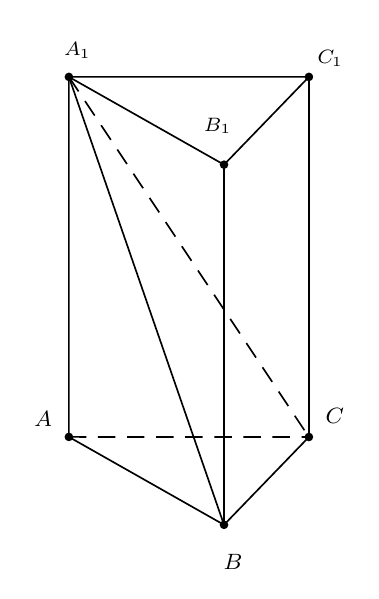
\begin{tikzpicture}[x=1mm,y=1mm,line width=0.210mm,line join=bevel,
  every node/.style={inner sep=0pt,outer sep=0pt}]
  % 缩档轮 0910：本图为「字大图不大」型——置宽 41.1mm 不动（几何外廓 31.62mm 本已在 27.7–36mm 档内），
  %   只把标签字号 ×0.4584 到 7.5pt 档（见 缩档测量/缩档测量.txt【一】g1 行）。线宽同轮按
  %   「0.21 ÷ 有效系数（本图 41.1/41.100＝1.000）」改声明为 0.210mm。
  % 下标随主档同缩：宿宏 \qldsub 内嵌 9.68pt 定档、\qldrop 定坠 0.649mm 均不随节点字号缩，
  %   若不同步覆写则下标「1」(9.84pt) 反比主字母 (6.94pt) 大、且落正文档 [9.6,11.2] 被误判为正文行。
  %   覆写限本 tikzpicture 组内（\qldrop 0.649×0.4584＝0.2975mm／9.68×0.4584＝4.44pt），qp-blocks.tex 未动。
  \renewcommand{\qldrop}{0.2975mm}%
  \renewcommand{\qldsub}[1]{\raisebox{-\qldrop}{\fontsize{4.44pt}{4.44pt}\selectfont $#1$}}%
  % line join=bevel：源图角部无 miter 尖刺（A1 处两线交角 29.5°，miter 会长出 1.45mm，源图实测无）
  \path[use as bounding box] (0,0) rectangle (41.100,68.936);  % 源画布 691×1159px
  % ---- 顶点：10 条边逐线亚像素拟合后取交点（残差 <0.16px）；注释为源图像素坐标 ----
  \coordinate (A1) at ( 5.235,62.684);  % px( 88.008, 105.125)
  \coordinate (C1) at (35.717,62.684);  % px(600.498, 105.117)
  \coordinate (B1) at (24.936,51.534);  % px(419.239, 292.585)
  \coordinate (A)  at ( 5.234,16.961);  % px( 87.997, 873.843)
  \coordinate (C)  at (35.717,16.952);  % px(600.495, 873.999)
  \coordinate (B)  at (24.935, 5.798);  % px(419.225,1061.522)
  % ---- 线网：上底三边实线；三条侧棱实线；下底 AB、BC 实线、AC 虚线（被遮棱）；A1B 实线辅助线；CA1 虚线辅助线
  \draw (A1) -- (C1) -- (B1) -- cycle;
  \draw (A1) -- (A);
  \draw (B1) -- (B);
  \draw (C1) -- (C);
  \draw (A) -- (B) -- (C);
  \draw[dash pattern=on 2.214mm off 1.480mm] (A) -- (C);
  \draw (A1) -- (B);
  \draw[dash pattern=on 2.214mm off 1.480mm] (A1) -- (C);
  % ---- 六顶点实心点（半径 0.548mm＝源墨 0.531mm 扣口径校正）----
  \foreach \p in {A1,C1,B1,A,C,B} \fill (\p) circle[radius=0.548mm];
  % ---- 标签：anchor=base（y＝源图基线；x＝主体字墨心，均按源图墨 bbox 标定，偏差 <0.06mm）----
  % 字号档（缩档轮 0910）：主体 17.30→7.93pt、带下标档 14.90→6.83pt（均 ×0.4584＝7.5÷中位 16.36）
  %   → 件内渲染 8.06／6.94pt，中位 7.50pt 命中 TW-05 目标；两档固有档差 2.44pt 系源图标定，非本轮引入。
  %   第二参（行距 17/20pt）对 anchor=base 的单行节点不起作用，按「只改字号档」的最小改动原则保留原值。
  \node[anchor=base,font=\fontsize{6.83pt}{17pt}\selectfont] at ( 6.226,65.363) {\qlabs{A}{1}{-0.117mm}}; % 源 px 基线 y=59 ,  墨心 x=87.0
  \node[anchor=base,font=\fontsize{6.83pt}{17pt}\selectfont] at (38.333,64.350) {\qlabs{C}{1}{-0.308mm}}; % 源 px 基线 y=77 ,  墨心 x=634.5
  \node[anchor=base,font=\fontsize{6.83pt}{17pt}\selectfont] at (24.037,55.768) {\qlabs{B}{1}{-0.096mm}}; % 源 px 基线 y=221,  墨心 x=389.0
  \node[anchor=base,font=\fontsize{7.93pt}{20pt}\selectfont] at ( 1.979,18.325) {\qlab{A}};                % 源 px 基线 y=850,  墨心 x=28.0
  \node[anchor=base,font=\fontsize{7.93pt}{20pt}\selectfont] at (38.991,18.712) {\qlab{C}};                % 源 px 基线 y=844,  墨心 x=657.0
  \node[anchor=base,font=\fontsize{7.93pt}{20pt}\selectfont] at (26.082, 0.063) {\qlab{B}};                % 源 px 基线 y=1157, 墨心 x=436.5
\end{tikzpicture}%
}\newpage
\resizebox{42.0mm}{!}{% g2-cubeE.tikz —— 片G 0910 集成自 _tmp片G素材/image2_重绘.tex（L18–53 片段正文，逐字拷入，仅末行加 %）
% 源图：variantF/media/media/image2.png 764×764px = 源排印宽 42.0mm
% 依赖：宿主导言 \usepackage{tikz}；\qon/\qoff 为片段内局部 \def，不入导言
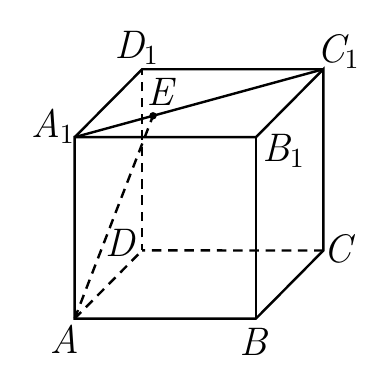
\begin{tikzpicture}[x=1mm,y=1mm,line width=0.308mm,line cap=butt,line join=miter,
                    every node/.style={font=\fontsize{14.53pt}{17.436pt}\selectfont}]
% ---- 坐标（mm，原点=位图左上角，y 向上） ----
\coordinate (A)  at (5.971,5.058);\coordinate (B)  at (28.993,5.058);
\coordinate (A1) at (5.971,28.092);\coordinate (B1) at (28.993,28.092);
\coordinate (C)  at (37.547,13.696);\coordinate (C1) at (37.547,36.723);
\coordinate (D)  at (14.543,13.713);\coordinate (D1) at (14.543,36.723);
\coordinate (E)  at (15.917,30.809);   % E = 线 A1C1 ∩ 线 AE（源图 t=0.315，见核对表）
% ---- 虚线（隐藏棱 AD、DC、DD1 与辅助线 AE）----
\def\qon{1.209mm}\def\qoff{0.852mm}
\draw[dash pattern=on \qon off \qoff, dash phase=0.033mm] (A)--(D);    % 首段墨迹距 A 36.9px
\draw[dash pattern=on \qon off \qoff, dash phase=0.825mm] (D)--(C);    % 自 D 起 22.5px 起墨
\draw[dash pattern=on \qon off \qoff, dash phase=0.399mm] (D)--(D1);   % 相位按 dash 中心拟合（自 D 起第1段中心 30.25px）
\draw[dash pattern=on \qon off \qoff, dash phase=0.049mm] (A)--(E);    % 首段墨迹距 A 36.6px
% ---- 实线：前面 ABB1A1、右面 BCC1B1、上面 A1B1C1D1、对角线 A1C1 ----
\draw (A)--(B)--(C)--(C1)--(B1)--(A1)--(A)--cycle;   % 外轮廓：A-B、B-C、C-C1、C1-B1、B1-A1、A1-A
\draw (B)--(B1);                                     % 前面右竖棱 B-B1
\draw (A1)--(D1)--(C1);                              % 上面后两条可见棱
\draw (A1)--(C1);                                    % 上面对角线（E 所在）
% ---- 点 E（实心圆）----
\fill (E) circle[radius=0.472mm];
% ---- 标签 ----
\node at (4.644,2.350) {$\mathit{A}$};
\node at (28.898,2.116) {$\mathit{B}$};
\node at (39.683,13.844) {$\mathit{C}$};
\node at (11.954,14.713) {$\mathit{D}$};
\node at (17.085,33.897) {$\mathit{E}$};
\node at (3.229,29.422) {$\mathit{A}_{\mathrm{1}}$};
\node at (32.520,26.320) {$\mathit{B}_{\mathrm{1}}$};
\node at (39.457,38.888) {$\mathit{C}_{\mathrm{1}}$};
\node at (13.870,39.477) {$\mathit{D}_{\mathrm{1}}$};
% ---- 外框＝源排印幅面 42x42mm（与源位图 764x764px 同幅；不含图形，只定画布大小，
%      比节点自然外框（44.7x43.5mm）更贴源幅面。集成方若要“紧框”，删掉这两行即可） ----
\pgfresetboundingbox
\path[use as bounding box] (0,0) rectangle (42,42);
\end{tikzpicture}%
}\newpage
\resizebox{36.3mm}{!}{% g3-cube6.tikz —— 片G 0910 集成自 _tmp片G素材/tikz_tan6.tex（L27–68 片段正文，逐字拷入，仅删空行、末行加 %）
% 源图：variantF/media/media/image3.png 521×496px = 源排印 86.0×82.0mm
% 集成口径：本片按栏宽封顶置 84.0mm（源 86mm 略缩 2.3%，同比缩放，线宽/字号/虚线一并缩）
% 依赖：宿主导言 \usepackage{tikz} + \definecolor{cubegray}{gray}{0.25}（见 qp-blocks.tex）
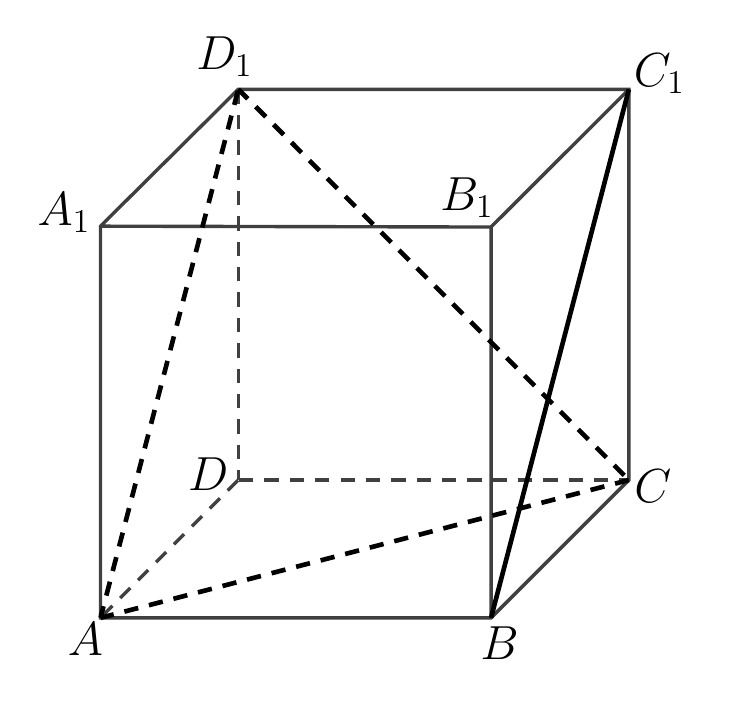
\begin{tikzpicture}[x=1mm,y=1mm,
    line width=0.43mm, line cap=butt, line join=miter,
    every node/.style={inner sep=0pt,outer sep=0pt},
    lab/.style={font=\fontsize{17.5}{21}\selectfont}]
  \useasboundingbox (0,0) rectangle (86,82);
  % ---- 顶点 ----
  \coordinate (A)  at ( 9.25, 7.05);
  \coordinate (B)  at (58.85, 7.05);
  \coordinate (C)  at (76.35,24.55);
  \coordinate (D)  at (26.75,24.55);
  \coordinate (A1) at ( 9.25,56.79);
  \coordinate (B1) at (58.85,56.68);
  \coordinate (C1) at (76.35,74.17);
  \coordinate (D1) at (26.75,74.17);
  % ---- 灰线·实线棱（9 段）----
  \draw[cubegray] (A)--(B)--(C)--(C1)--(D1)--(A1)--cycle % 底前棱、底右棱、右后棱、顶后棱、顶左棱、左前棱
                  (A1)--(B1)--(B)                        % 顶前棱、右前棱
                  (B1)--(C1);                            % 顶右棱
  % ---- 灰线·虚线棱（3 段隐藏棱：AD、DC、DD₁）----
  % dash phase = 按源图虚线节距逐段反解的对相（锚点=笔画起端；on 1.82 / off 1.40mm，周期 3.22mm）
  \draw[cubegray,dash pattern=on 1.82mm off 1.40mm,dash phase=2.90mm] (A)--(D);
  \draw[cubegray,dash pattern=on 1.82mm off 1.40mm,dash phase=0.62mm] (C)--(D);
  \draw[cubegray,dash pattern=on 1.82mm off 1.40mm,dash phase=3.18mm] (D1)--(D);
  % ---- 黑粗线（问题向量及其平移辅助：BC₁ 实线；AC、AD₁、D₁C 虚线）----
  \draw[line width=0.59mm] (B)--(C1);
  \draw[line width=0.59mm,dash pattern=on 1.82mm off 1.40mm,dash phase=0.09mm] (A)--(C);
  \draw[line width=0.59mm,dash pattern=on 1.82mm off 1.40mm,dash phase=0.30mm] (A)--(D1);
  \draw[line width=0.59mm,dash pattern=on 1.82mm off 1.40mm,dash phase=0.11mm] (D1)--(C);
  % ---- 顶点标签（位置 = 源图墨迹中心，mm）----
  \node[lab] at ( 4.62,58.48) {$A_1$};
  \node[lab] at ( 7.35, 4.38) {$A$};
  \node[lab] at (59.93, 3.80) {$B$};
  \node[lab] at (55.80,60.43) {$B_1$};
  \node[lab] at (80.22,76.13) {$C_1$};
  \node[lab] at (79.40,23.72) {$C$};
  \node[lab] at (22.94,25.29) {$D$};
  \node[lab] at (25.01,78.28) {$D_1$};
\end{tikzpicture}%
}\newpage
\resizebox{30.5mm}{!}{% g4-dihedral.tikz —— 片G 0910 集成自 _tmp片G素材/片G-image4-二面角.tikz（L22–58 正文，逐字拷入，仅删空行）
% 源图：variantF/media/media/image4.png 788×424px = 源排印宽 66.3mm；画布 66.3000×35.6741mm
% 集成口径：素材注记的 \resizebox{33.120mm}（侧绕排）作废，本片按源尺寸 66.3mm 图下置居中
% 依赖：宿主导言 \usepackage{tikz}
% 注：末行 % 必需——\input 时尾随换行会成空格 token，被计入裁切框（实测 +3.33pt 页宽）。
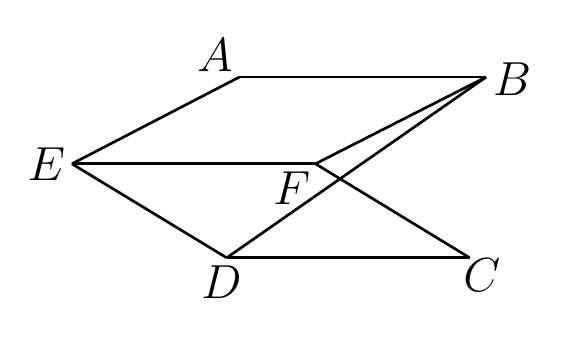
\begin{tikzpicture}[x=1mm,y=1mm,line width=0.34mm,line cap=butt,line join=miter,
                    font=\fontsize{16.03pt}{19.2pt}\selectfont]
  \path[use as bounding box] (0,0) rectangle (66.3000,35.6741);   % bbox＝源画布 788×424 px
  % ---- 顶点坐标（源 px 见行末注；由 8 条线最小二乘拟合并求交，残差 ≤0.6px） ----
  \coordinate (E) at ( 5.6204,18.3839);   % px(  66.80, 205.50)  EF∩EA
  \coordinate (A) at (26.8969,29.4059);   % px( 319.68,  74.50)  EA∩AB
  \coordinate (B) at (58.2228,29.4059);   % px( 692.00,  74.50)  AB∩FB（∩DB 得 690.87，取中）
  \coordinate (F) at (36.5491,18.3839);   % px( 434.40, 205.50)  EF∩FB（∩FC 得 435.56，取中）
  \coordinate (D) at (25.2748, 6.4470);   % px( 300.40, 347.375) ED∩DC（∩DB 得 299.17，取中）
  \coordinate (C) at (56.1463, 6.4470);   % px( 667.32, 347.375) DC∩FC
  % ---- 线（全实线，无箭头；逐条对应源图线要素） ----
  % 正方形 ABFE 四边：EF 下边、AB 上边、EA 左边、FB 右边
  \draw (E) -- (A);      % 左棱
  \draw (A) -- (B);      % 上边（源水平线 y=74.50px）
  \draw (E) -- (F);      % 公共棱 EF（源水平线 y=205.50px）
  \draw (F) -- (B);      % 右棱
  % 正方形 CDEF 四边：EF 公共棱（已画）、FC 右边、DC 下边、ED 左边
  \draw (E) -- (D);      % 左棱
  \draw (F) -- (C);      % 右棱
  \draw (D) -- (C);      % 下边（源水平线 y=347.375px）
  % 连线 BD（源图唯一交叉线：BD 与 FC 交于 px(471.4,227.4)＝mm(39.66,16.54)）
  \draw (B) -- (D);
  % ---- 标签（锚点＝源字母墨迹盒对应角，mm；inner sep=0 使锚点即字盒边） ----
  % 位置经三轮闭环标定：①按源墨迹盒角落位（残差=TeX 字盒宽/深≠墨迹盒，逐字不同）；
  % ②788px 帧互相关对齐（dx=dy=0.25px）后逐字修正；③以线网为基准逐字母亚像素微调
  % （2x 帧、0.5px@1x 步进，目标＝阈值 IoU 最大）——终态逐字母墨迹盒残差 ≤1px@1x（≤0.08mm）
  % 6 字母 + 线网的最优位移已完全一致（同为 (0,+1)px@2x），即无逐要素残余错位
  \node[anchor=south east,inner sep=0pt] at (26.1666,29.9950) {$A$};  % 源盒 px x[265,306] y[ 21, 66]
  \node[anchor=west,      inner sep=0pt] at (58.9380,29.1114) {$B$};  % 源盒 px x[702,741] y[ 57,101]
  \node[anchor=north west,inner sep=0pt] at (55.1518, 6.5206) {$C$};  % 源盒 px x[661,703] y[349,395]
  \node[anchor=north,     inner sep=0pt] at (24.6101, 5.5531) {$D$};  % 源盒 px x[268,315] y[360,404]
  \node[anchor=east,      inner sep=0pt] at ( 4.9220,18.2998) {$E$};  % 源盒 px x[ 12, 54] y[185,229]
  \node[anchor=north,     inner sep=0pt] at (33.5285,17.5847) {$F$};  % 源盒 px x[377,419] y[217,261]
\end{tikzpicture}%
}\newpage
\resizebox{28.2mm}{!}{% g5-fold.tikz —— 片G 0910 集成自 _tmp片G素材/fig-image5-fold-body.tex（L36–65 正文，逐字拷入）
% 源图：variantF/media/media/image5.png 1798×1350px = 源排印宽 54.7mm
% 集成口径：本片仍 \resizebox{54.7mm}{!}{…}（同比缩放＝素材认可的安全法）。
%   本片段无 bbox 锁定，自然外框含标签外扩（源图 C 标签右端被画布裁去，本稿按完整字形放置），
%   故实测宽略大于 54.7mm 的图形部分会被同比缩 ~3.3%（登记项）。
% 依赖：宿主导言 \usepackage{tikz}；im5dash 为本片段内 tikz key，不入导言
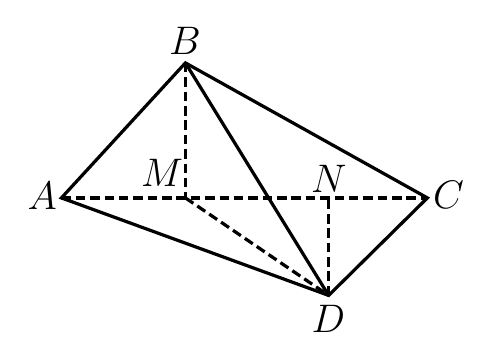
\begin{tikzpicture}[
  x=1mm, y=1mm,
  % 缩档轮 0910：置宽 54.7→28.2mm（标签渲染 14.55→7.50pt 命中 TW-05 目标，字号档 14.4pt 不动、随同比缩）。
  %   本片段无画布锁定 → 有效系数取实测反推：现 0.3025mm÷声明 0.3042mm＝0.99441，
  %   新 0.99441×(28.2÷54.7)＝0.51266 → 声明回填 0.21÷0.51266＝0.4096mm。
  line width=0.4096mm,
  line cap=butt, line join=miter,
  im5dash/.style={dash pattern=on 1.2169mm off 0.6085mm},
  every node/.style={inner sep=0pt, font=\fontsize{14.4pt}{14.4pt}\selectfont}
]
  % ---- 顶点 ----
  \coordinate (A) at ( 3.9650,18.6187);
  \coordinate (B) at (19.7139,35.7637);
  \coordinate (C) at (50.4429,18.6187);
  \coordinate (D) at (37.9027, 6.2360);
  \coordinate (M) at (19.7139,18.6187);
  \coordinate (N) at (37.9027,18.6187);
  % ---- 实线：两个三角形的边 + 折起后 BD ----
  \draw (A) -- (B) -- (C) -- (D) -- cycle;
  \draw (B) -- (D);
  % ---- 虚线：对角线 AC、垂线 BM、垂线 DN、MD（源图 M–D 亦为虚线） ----
  \draw[im5dash] (A) -- (C);
  \draw[im5dash] (B) -- (M);
  \draw[im5dash] (D) -- (N);
  \draw[im5dash] (M) -- (D);
  % ---- 标签（西文斜体数学体，anchor=center 对准源图字形中心） ----
  \node at ( 1.5363,18.8164) {$A$};
  \node at (19.6531,38.5101) {$B$};
  \node at (53.1180,18.9686) {$C$};
  \node at (37.8763, 3.2552) {$D$};
  \node at (16.7477,21.8435) {$M$};
  \node at (37.9219,21.0981) {$N$};
\end{tikzpicture}%
}
\end{document}
